\documentclass[12pt]{report}
\usepackage[font=small, labelfont=bf]{caption}
\usepackage[english]{babel}
\usepackage{sectsty}
\usepackage{float}
\usepackage{amsmath}
\usepackage{siunitx}
\usepackage{graphicx} % For plots

%%% Custom Settings %%%
\renewcommand{\thesection}{\arabic{section}}        % Change section numbering ( 0.1 -> 1 )
\setcounter{tocdepth}{3}                            % Include subsubsections in ToC
\setcounter{secnumdepth}{3}
\sisetup{mode=text,range-phrase = {\text{~to~}}}    % Change range ( atob -> a to b )
\newcommand\tab[1][1cm]{\hspace*{#1}}               % Use tabs
\newcommand{\dd}[1]{\mathrm{d}#1}                   % Integral's dd

\title{ \normalsize \LARGE {\uppercase{Digital Modulation Simulation Project}}}
\author{
    Brian Doan \\ Derek Lee \\ Steven Lee \\\\ 
    Professor Frost \\ Communication Theory 
}
\date{November 15, 2020}

\begin{document}

\maketitle
\tableofcontents
\newpage

%%%%%%%%%%%%%%%%%%%%%%%%%%%%%%%%%%%%%%%%%%%%
\section{Introduction}

\tab This project explores three different digital modulation schemes and their performance with additive white Gaussian noise on MATLAB. The symbols transmitted by these schemes are estimated using the least squares decision metric. Digital communication systems are typically defined by a two dimensional constellation of symbols. The effect of noise is analyzed through I/Q decomposition of the transmitted symbols, which does not require integration. Instead, the least squares decision metric was reduced to the minimum distance between two points on a plane. To evaluate performance under the effect of noise, the simulation plots the probability of error against the SNR per bit.

\quad The three digital modulation systems in the simulation were Phase Shift Keying (PSK), Differential Phase Shift Keying (DPSK) and Quadrature Amplitude Modulation (QAM). 

\quad PSK encodes the symbols in the phase of the signal itself, which can be generated using a typical I/Q decomposition. The symbols are equidistant and have the same energy. This project evaluates the performance of each scheme under the effect of additive white Gaussian noise. In DPSK, the carrier phase is shifted relative to the high or low of the previous state. QAM uses a constellation with symbols obtained from combining two carriers that are 90 degrees apart. QAM allows for any shape but is usually a square. In the M=32 case, the simulation used a tall rectangle. 

\newpage

%%%%%%%%%%%%%%%%%%%%%%%%%%%%%%%%%%%%%%%%%%%%
\section{Methods}


\tab The script functions were timed with the `tic' and `toc' commands to evaluate efficiency. The implementation of the Least Squares algorithm does not use a for loop. Instead, the function uses vectorization to compute the magnitude of the distances between the randomly generated noisy symbols with the constellation vector. The minimum distance corresponds with the closest point on the constellation. A script function was used to randomly generate symbols from a constellation by randomly sampling with replacement. Taking advantage of the Least Squares method simplification was more efficient than taking an integral and using loops.

\quad The `calcError' function similarly uses vectorization to avoid the use of for loops to calculate the error between the true transmitted symbols and the predicted received symbols. A low threshold value of $\num{e-3}$ was used to account for machine precision. Any instances greater than the threshold value were detected with the `nnz' MATLAB function. The output value was the percent error. \\

\noindent The following formula was used to calculate the Desired Average Energy:
\begin{equation}
    E_S = SNR/bit * N_o * \log_2(M)
\end{equation}
This formula was used to scale the constellation to the true constellation with the correct average energy.

\quad The `scaleNonDiff' function avoids the use of loops by taking advantage of the efficiency of the implementation of Least Squares. The function directly takes in the scaled constellation and additive complex noise to calculate an estimated system. The complex noise was generated from zero-mean Gaussian at half noise power to include both real and imaginary noise.

\quad The `scaleDiff' function is similar to the `scaleNonDiff' function. The difference is the use of angles. The constellation used for DPSK is generated from taking the phase differences of the true constellation. The noise-free symbols were generated in a similar manner. The noisy symbols were generated by taking the phase differences of the true noise-free symbols combined with noise.

\newpage

%%%%%%%%%%%%%%%%%%%%%%%%%%%%%%%%%%%%%%%%%%%%
\section{Results}

All of the following schemes were evaluated with:
\begin{itemize}
    \item $N = \num{e5}$ symbols
    \item $N_o = 10$
    \item $SNR/bit = \SIrange{-4}{20}{dB}$ with 1 dB resolution
\end{itemize}

\begin{table}[H]
    \centering
    \begin{tabular}{|| c | c | c ||} 
    \hline
        Question & Method & Time (sec) \\ [0.5ex]
        \hline
        1 & Least Squares & 0.009934 \\
        \hline
        2-4 & Non-Differential \& Differential & 0.023222 \\
        \hline
        5 & Binary Antipodal \& Binary Orthogonal & 0.436630 \\
        \hline
        6 & M-ary PSK & 1.265682 \\
        \hline
        7 & M-ary DPSK & 1.358170 \\
        \hline
        8 & M-ary QAM & 1.910961 \\
        \hline
    \end{tabular}
    \caption{Running times for each question}
    \label{tab:Run Times}
\end{table}

\newpage

%%%%%%%%%%%%%%%%%%%%%%%%%%%%%%%%%
\subsection{Binary Signaling}

\begin{figure}[!htb]
    \begin{center}
    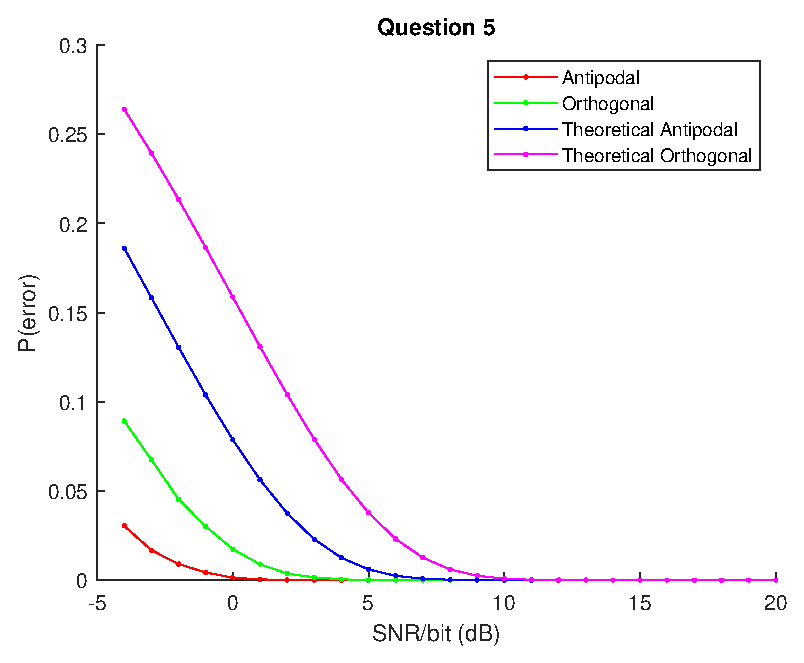
\includegraphics[scale=1]{Question5}
    \caption{Plot of Probability of Error vs SNR/bit}
    \end{center}
\end{figure}

\newpage

%%%%%%%%%%%%%%%%%%%%%%%%%%%%%%%%%
\subsection{M-ary Signaling}

The M-ary PSK and DPSK schemes were evaluated for $M = \{ 4, 8, 16, 32 \}$. \\
The M-ary QAM scheme was evaluated for $M = \{ 4, 16, 32, 64 \}$.

%%%%%%%%%%%%%%%%%%%%%%
\subsubsection{PSK}

\begin{figure}[!htb]
    \begin{center}
    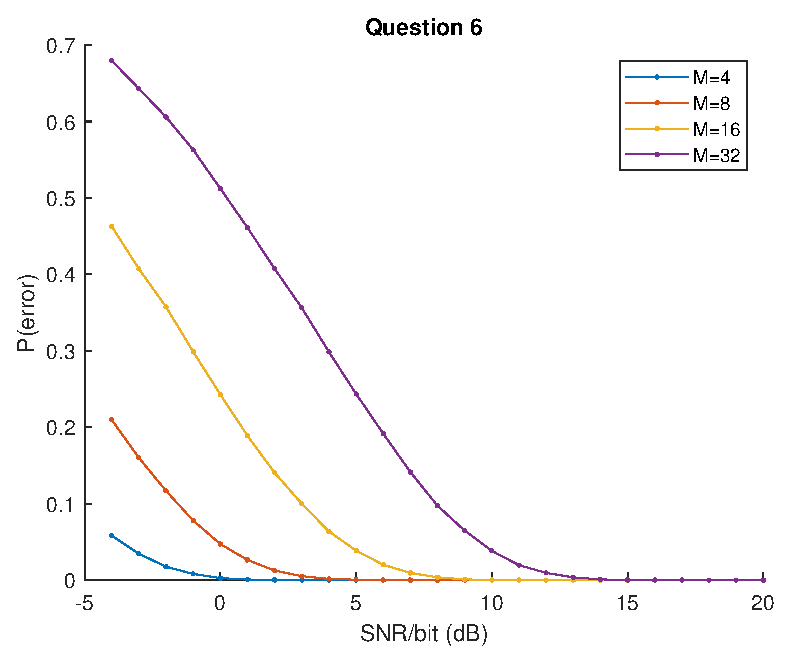
\includegraphics[scale=1]{Question6}
    \caption{Plot of Probability of Error vs SNR/bit}
    \end{center}
\end{figure}

\newpage

%%%%%%%%%%%%%%%%%%%%%%
\subsubsection{DPSK}

\begin{figure}[!htb]
    \begin{center}
    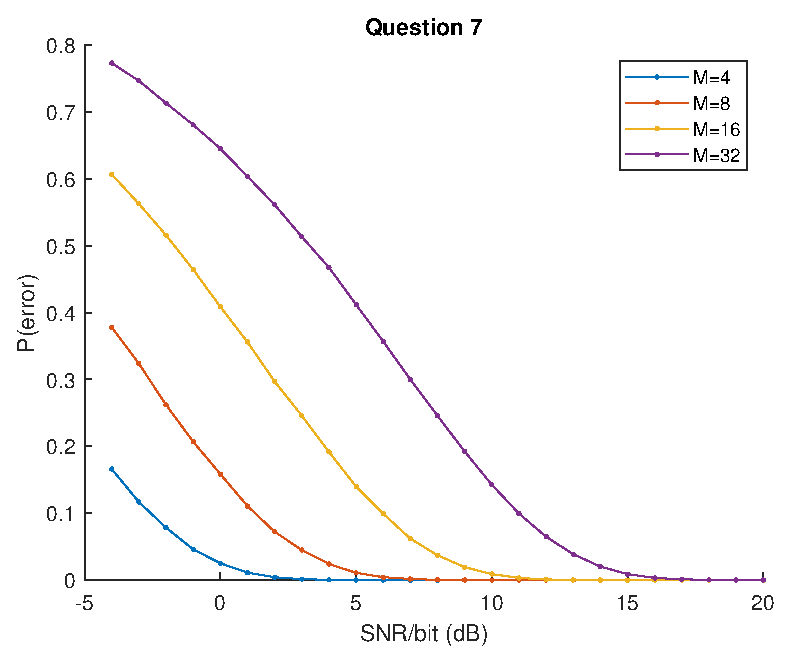
\includegraphics[scale=1]{Question7}
    \caption{Plot of Probability of Error vs SNR/bit}
    \end{center}
\end{figure}

\newpage

%%%%%%%%%%%%%%%%%%%%%%
\subsubsection{QAM}

\begin{figure}[!htb]
    \begin{center}
    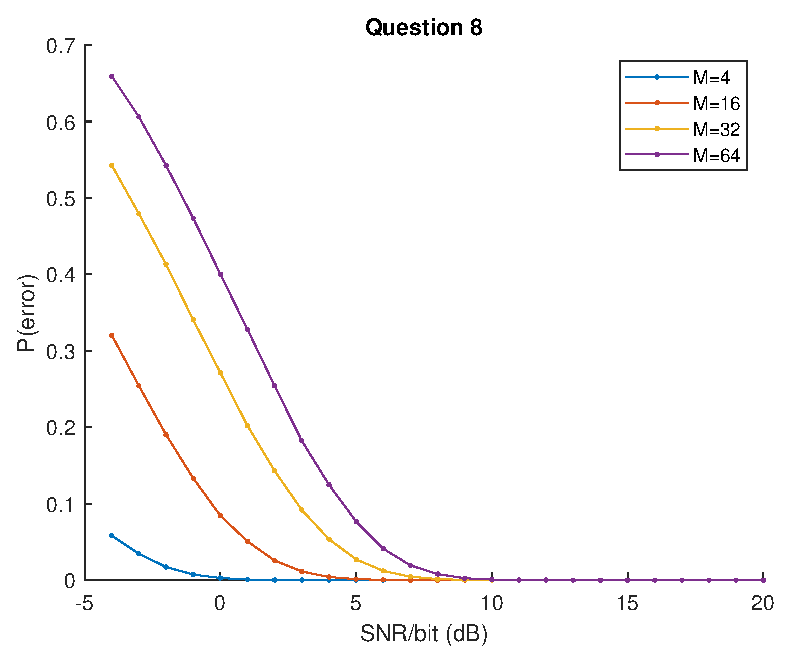
\includegraphics[scale=1]{Question8}
    \caption{Plot of Probability of Error vs SNR/bit}
    \end{center}
\end{figure}

\newpage

%%%%%%%%%%%%%%%%%%%%%%%%%%%%%%%%%%%%%%%%%%%%
\section{Discussion}

\tab For the entire program, $\num{e5}$ symbols were generated. Table 1 displays the run times for each part of the simulation. The M-ary sections take longer than the binary signaling since binary signaling is the special case where M = 2. The DPSK takes longer than the PSK since it requires more computation to calculate the phase differences. QAM takes the longest since M = 64 is computed instead of M = 8 in the PSK section.

\quad To generate the noise, the variance of the real and imaginary parts was half of the variance given by the noise power. This was based on the theorem for linear combinations of Gaussian random variables.

\quad Testing the Least Squares function (`LSNonDiff') took 0.009934 seconds. This is reasonable since the function just a takes difference and finds the constellation point with the index of the minimum difference.

\quad Testing the non-differential and differential functions (`scaleNonDiff', `scaleDiff', and `calcError') took 0.023222 seconds. The `scaleNonDiff' function takes a base constellation, a list of N noise-free transmitted symbols, a value for noise power and a desired SNR per bit. The desired average symbol energy is calculated using Equation 1. The value that the constellation is scaled by is calculated using the square root of the desired average symbol energy divided by the average energy of the constellation. This value is used to form the true constellation. Initially, a noise power of 1 was used. However, the noise power was later changed to 10, because it led to better results. Next, the noise is generated and is added to the symbols. The predicted values of the transmitted symbols is computed using the LS decision metric. The `scaleDiff' function is similar to the `scaleNonDiff' function, but it uses phase differences by computing the difference between two adjacent symbols and computing the arc-tangent of the ratio between the imaginary part and the real part of those differences. The constellation and the symbols are transformed from a range of $-\pi to \pi$ to $0 to 2\pi$. Then, in the `LSDiff' function, the angle constellation is combined with a copy of itself with $2\pi$ is added to it. This ensures the least squares decision metric will work properly with wrapped angles (e.g. $2\pi$ is equivalent to 0).

\quad In the binary antipodal and binary orthogonal simulations, the theoretical probability of error was calculated using the `qfunc' MATLAB function. The Q function is an integral from x to infinity of a decreasing function that is 1/2 at x = 0. It is defined as follows:

\begin{equation}
    \int_{x}^{\infty} \frac {1}{2\pi} \exp(\frac {-t^2}{2}) \dd{t}
\end{equation}

\noindent The expression inside the integral is the tail of the standard normal distribution. The Q function evaluates the probability of the positive tail. The two symbols in the binary antipodal constellation have a phase difference of 180 degrees, while the two symbols in the binary orthogonal constellation have a phase difference of 90 degrees.

%The minimum bit error probabilities are bounded by the exponential part of the Q function definition. This means that with an increasing signal to noise ratio, the error probability will decrease exponentially.
 
\quad The experimental part of the simulation used the `probErrorNonDiff' function for both types of binary signaling. Throughout the entire simulation, the theoretical values for the probability of error are higher than the experimental values. This is probably due to an assumption made to compute the theoretical values that is not true in the implementation of the schemes. This may also be due to an error in the implementation.

\quad For M-ary schemes, the symbols are $\frac {2\pi}{M}$ apart. In the `genM\_ary' and `genQAM' functions, M evenly spaced symbols are generated. As M increases for these schemes, naturally, the bandwidth efficiency increases. A higher M also increases the probability of error. A higher SNR is required to reach 0\% error. This is because the distances between the symbols are smaller, which increases the effect of noise on the received symbols.

\quad The differential scheme for PSK has a higher probability of error than its non-differential counterpart. This result is expected because each DPSK symbol is dependent on the accuracy of two symbols, rather than just one symbols. This is because DPSK is computed using the relative differences between two adjacent symbols, rather than PSK, which directly uses each symbol. The noise in both of the symbols is compounded, meaning the noise will have a larger effect on the differential scheme compared to the non-differential scheme.

\quad For the quadrature amplitude modulation scheme, the carriers (the cosines and sines) are modulated and added together to obtain a signal. A tall rectangular constellation was generated for M values that were not perfect squares. One dimension of the rectangle was computed by taking the floor of the square root of the M value. The second dimension was computed by taking the quotient of M and the first dimension. The constellation was centered at the origin based on these two dimensions. The probability of error for this scheme decreases at a steeper slope compared to the other schemes for the same M values.

\quad Of the three digital modulation schemes, QAM performs the best across the range of SNR values used for this project, while DPSK performs the worst. The 4-QAM and the 4-PSK have similar performance, but for $M > 4$, QAM performs better. This is reasonable because QAM modulates in both phase and amplitude. The cost here would be in the increase in the required SNR to achieve a desired bit error. The minimum distance between adjacent symbols affects the probability of error. In DPSK and PSK, the distances are smaller, which increases error. In QAM, the distance is larger, so there would be a lower bit error.

\newpage

%%%%%%%%%%%%%%%%%%%%%%%%%%%%%%%%%%%%%%%%%%%%
\section{Acknowledgements}
We would like to acknowledge:
\begin{itemize}
    \item Brian Frost for teaching us Communication Theory 
    \item Thodori Kapouranis for pointing out an error in our scaling functions
    \item Joshua Yoon for comparing results with us on this project
\end{itemize}

\newpage


\end{document}
